\documentclass[a4paper,12pt]{report}
\usepackage[utf8]{inputenc}
\usepackage{graphicx}
\begin{document}
\begin{titlepage}
\begin{center}
    \vspace*{1cm}
    
    \Huge
    \textbf{Computer Music Languages and Systems}
    
    \vspace{0.5cm}
    \LARGE
    Homework n° 1, audio effect classification

    \vspace{1 cm}
    
    \textbf{Giovanni Affatato}
    
    \vspace{0.5cm}
    
    \textbf{Davide Lionetti}
     
    \vspace{0.5cm}
    
    \textbf{Luca Cattaneo}
     
    
    \vspace{0.5cm}
    
    \textbf{Jonathan "Bho"}
    
    \vspace{0.5cm}
    
    \vfill
    % Report for the second homework of the Digital Audio Analysis and Processing module of the SASP course.
    
   
    \date{April 2021}
    \vspace{0.3cm}
    \textbf{Master of Science in Music and Acoustic Engineering}
    
    \vspace{0.8cm}
    
    
\includegraphics[width=0.5\textwidth]{logo_positivo.png}
    
\end{center}
\end{titlepage}


\abstract{}
Our group worked on \textbf{Assignment 3}: implement a 			  	classifier system able to predict the audio effect used in 			 	recordings of electric guitar and bass. We divided our work in 		 	steps as presented in the sections of this document, from the  	      	choice of the feature through the selection of a classification 		method, for each phase we present the decisions we made. In 			general, we used as a reference the second laboratory on 				Classification, mainly because we implemented the Support Vector 	Machine with majority voting for multiclass classification.
\endabstract{}

\chapter{Reasoning and implementation}
\section{Feature choice}
Due to the fact that both these effects imply a significant change in the power spectrum, It is efficient to use  as decision feature the Root Mean Square, that leads to good predictions.
\section{Dataset selection}
For the definition of the datasets, we decided to use only \textit{monophonic bass} and \textit{monophonic guitar} from \textbf{IDMT-SMT-AUDIO-EFFECTS} in order to have more homogeneous sample's features. While for the train and test sets we divided the whole classes in about half, as shown in the following table:

\begin{table}[!h]
\centering
\begin{tabular}{|c|c|c|}
\hline
           & \begin{tabular}[c]{@{}c@{}}Train\\ (\# elem)\end{tabular} & \begin{tabular}[c]{@{}c@{}}Test\\ (\# elem)\end{tabular} \\ \hline
Distortion & 1394                                                      & 1238                                                     \\ \hline
Tremolo    & 1194                                                      & 1228                                                     \\ \hline
NoFX       & 559                                                       & 555                                                      \\ \hline
\end{tabular}
\caption{Train and test datasets sizes}
\label{tab:my-table}
\end{table}

\section{Multi-class Weighted Support Vector Machine}
SVMs are generally binary classifier, so, in order to manage 3 classes, we used one SVC for each couple of class: Distortion/Tremolo, Distortion/NoFX and Tremolo/NoFX. Each one misclassify the missing class, hence, applying majority voting, we are able to train and test the SVM with all the instances of the samples.

In our training set we face the problem of having an unbalance amount of tracks for every class type. It contains half of no-effect tracks compared to the effected ones, hence we have found a way to solve this problem. The SVM model works well also with unbalanced training-set taking care of setting efficiently the right value of an internal private variable called C.\\ C  determines the number of tolerated severity apply to the margin violation (and to the hyperplane), it controls the trade-off between maximizing the separation margin between classes minimizing the number of misclassified instances.
Specifically, each example in the training dataset has its own penalty term C used in the calculation of the margin when fitting the SVM model. The value of an example’s C-value can be calculated as a weighting of the global C-value, where the weight is defined proportional to the class distribution. 

$$C_i = weight_i * C$$
By default it is suppose a balanced training-set, each class has the same weighting, which means that the softness of the margin is symmetrical.\\ A larger weighting factor C can be used for the minority class, allowing the margin to be softer (smaller penalty for misclassified examples), whereas a smaller C can be used for the majority class, forcing the margin to be harder and preventing misclassified examples.
This has the effect of encouraging the margin to contain the majority class with less flexibility, but allow the minority class to be flexible with misclassification of majority class examples onto the minority class side if needed.

\section{Cross-validation for SVM parameters}
In order to select appropriate parameters for the SVM, we tested our classifier through Cross-validation using the function GridSearchCV from scikit-learns, in doing so we were able to fine-tune the machine learning algorithm and to avoid overfitting the model. We decided also to run the grid-search only on the classifier between Tremolo and NoFX, because those were the classes that would presents more problems during the classification. The code snippet and the result is shown below, the score measures are precision and recall, while the C parameters were chosen arbitrarily within an order of magnitude:
\begin{verbatim}
tuned_parameters = [
  {'C': [1, 10, 100, 1000], 'kernel': ['linear']},
  {'C': [1, 10, 100, 1000], 'kernel': ['rbf']},
 ]

scores = ['precision', 'recall']

for score in tqdm(scores):
    print("# Tuning hyper-parameters for %s" % score)
    print()

    clf = GridSearchCV(
        SVC(), tuned_parameters, scoring='%s_micro' % score
    )
    clf.fit(X_train12, y_train_12)

    print("Best parameters set found on development set:")
    print()
    print(clf.best_params_)
    [...]
\end{verbatim}
\hfill \break
\textbf{Output:}

\begin{verbatim}
# Tuning hyper-parameters for precision

Best parameters set found on development set:

{'C': 1000, 'kernel': 'rbf'}

Grid scores on development set:

0.759 (+/-0.121) for {'C': 1, 'kernel': 'linear'}
0.735 (+/-0.073) for {'C': 10, 'kernel': 'linear'}
0.710 (+/-0.103) for {'C': 100, 'kernel': 'linear'}
0.689 (+/-0.085) for {'C': 1000, 'kernel': 'linear'}
0.916 (+/-0.044) for {'C': 1, 'kernel': 'rbf'}
0.984 (+/-0.035) for {'C': 10, 'kernel': 'rbf'}
0.993 (+/-0.019) for {'C': 100, 'kernel': 'rbf'}
0.993 (+/-0.016) for {'C': 1000, 'kernel': 'rbf'}
[...]

# Tuning hyper-parameters for recall

Best parameters set found on development set:

{'C': 1000, 'kernel': 'rbf'}

Grid scores on development set:

0.759 (+/-0.121) for {'C': 1, 'kernel': 'linear'}
0.735 (+/-0.073) for {'C': 10, 'kernel': 'linear'}
0.710 (+/-0.103) for {'C': 100, 'kernel': 'linear'}
0.689 (+/-0.085) for {'C': 1000, 'kernel': 'linear'}
0.916 (+/-0.044) for {'C': 1, 'kernel': 'rbf'}
0.984 (+/-0.035) for {'C': 10, 'kernel': 'rbf'}
0.993 (+/-0.019) for {'C': 100, 'kernel': 'rbf'}
0.993 (+/-0.016) for {'C': 1000, 'kernel': 'rbf'}
[...]
\end{verbatim}
\newpage
\chapter{Result}

In order to control the effectiveness of the feature, we first compared the plots of the rms of the three different classes. In these figures we saw that the \emph{distortion} effect has a long sustain phase, meanwhile \emph{NoFX} and \emph{tremolo} rapidly decay. These last two classes rms has the same envelope but \emph{tremolo} has an oscillating behaviour due to its characteristic amplitude oscillation.\\

\begin{figure}[h]
\centering
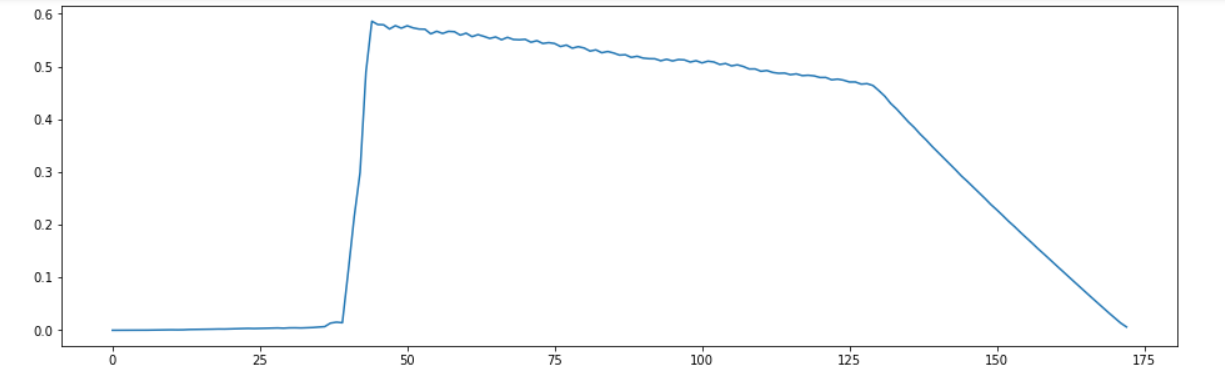
\includegraphics[scale=.2]{distortion.png}
\caption{Distortion}
\end{figure}
\begin{figure}[h]
\centering
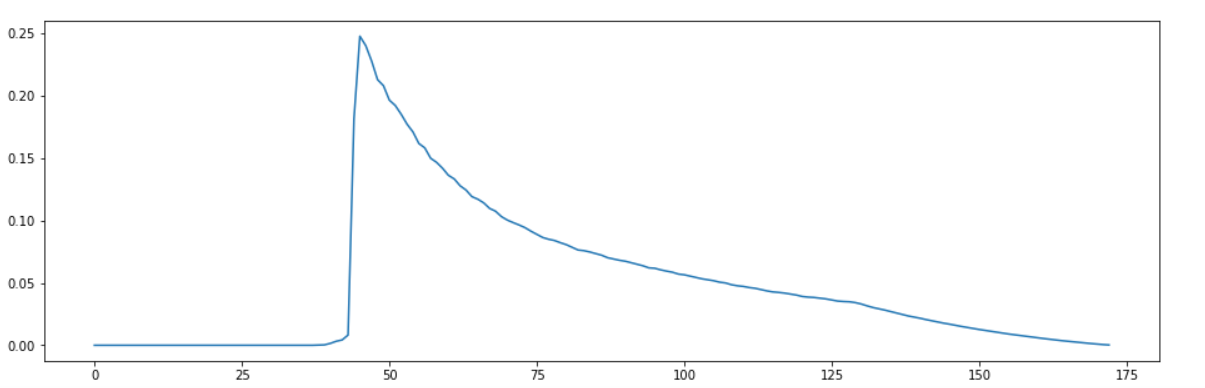
\includegraphics[scale=.2]{nofx.png}
\caption{No Effects}
\end{figure}
\begin{figure}[!h]
\centering
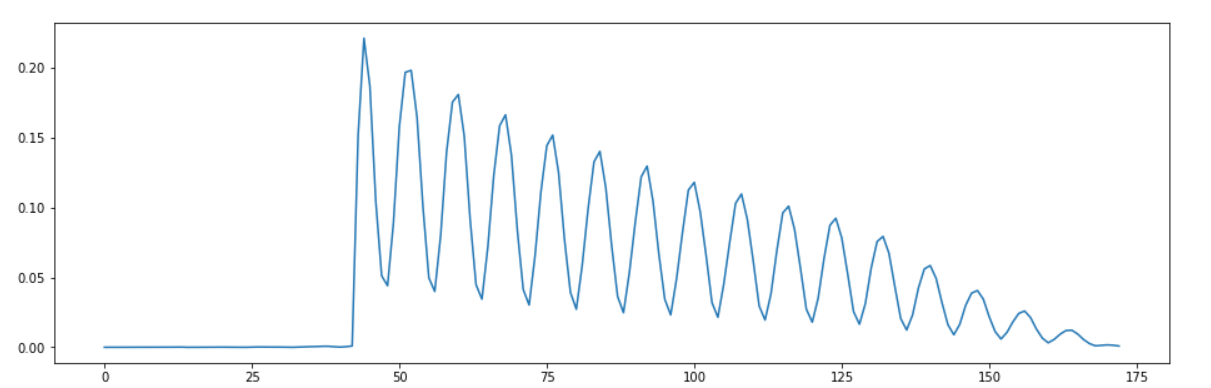
\includegraphics[scale=.2]{tremolo.png}
\caption{Tremolo}
\end{figure} 

We also compared the train and test set of the audio samples belonging to the same class and we saw that the rms are very similar to each other.\\
Then, at the end of the feature computation and voting we calculated and visualised the confusion matrix:
\begin{center}
\begin{tabular}{|c|c|c|c|}
	\hline
	  & distortion & tremolo & NoFx \\
	\hline
	distortion & 1219 & 19 & 0 \\
	\hline
	tremolo & 4 & 1224 & 0 \\
	\hline
	NoFX & 7 & 1 & 547  \\
	\hline
\end{tabular}
\end{center}

As the table above shows, the rms it is enough for a good separation and then identification of the three different effects, meanwhile using the other features we took in consideration. In particular with the others classifications \emph{tremolo} and \emph{NoFx} were quite confused each other.

\end{document}
